% !TEX root = ../main.tex
% !TEX program = xelatex
\section{问题分析}

四个问题围绕购电与储能的协调展开，区别在于决策时掌握的信息和允许调整的范围。问题一研究供需与电价已知时的安排；问题二加入供需预测误差；问题三利用日内信息调整订单；问题四进一步考虑未知的波动电价。各问共享电量平衡和储能约束，再针对新增条件扩展决策方法。

\subsection{问题一的分析}
问题一的关键是\textbf{供需与电价在时间上的错位}。光伏充足时未必用电最多，用电高峰也未必对应最低电价。储能可以转移电量，但容量、充放电功率和能量损耗限制了这种转移：提前充满可能挤占后续光伏的储存空间，过早放电又可能使高价时段缺少可用电量。因此，需要统筹全天的购电与充放电。

购电费用、电量平衡和储能变化均可用线性关系表示，适合用\textbf{电量流线性规划}求解。日初与日末储电量相等，则使每日安排能够重复执行，避免通过消耗初始库存压低当天费用。

\subsection{问题二的分析}
问题二在零点订电时尚不知道当天真实供需，需要先利用历史数据形成判断。负载具有星期规律，光伏的日际变化更强，因此二者应当\textbf{分别预测}。

预测偏差会造成两类损失：订电不足可能触发五倍电价的紧急补购，订电过多又可能付费后用不完。电池能够缓冲部分偏差，但受库存和功率限制。因此，需要根据近期误差设置适量准备，并考虑当天余电对次日购电的影响，将预测、误差准备和跨日调度结合起来。

\subsection{问题三的分析}
问题三允许获得新预报后修改尚未执行的订单。新光伏预报和已发生的负载可以修正零点判断，但短时偏差未必持续，部分缺口也可以由电池补足。因此，调整的关键是判断\textbf{未来供需变化是否值得支付改单费用}。

据此，将官方光伏预报与历史信息融合，利用当天负载偏差修正后续需求，再根据实际储电量滚动优化剩余订单。评价日内预报的价值时，应在相同调整权限下比较有、无后发预报的结果，区分新预报的收益与反馈改单本身的收益。

\subsection{问题四的分析}
问题四中，未来电价也需要预测。价格判断会改变提前购电和储能转移是否合算，因此应将\textbf{价格预测纳入调度}，而不只是更换最终结算单价。

两条分支分别承接问题二和问题三。零点分支主要依靠历史价格与供需特征判断全天价格；日内分支还可利用当天已发生的价格修正后续判断。针对两种信息条件分别选择预测方法，再将预测价格用于决策、实际价格用于结算，以评价价格预测对购电安排的实际作用。

四问的模型组成及递进关系如图~\ref{fig:overall_model_framework}所示。
\begin{figure}[H]
\centering
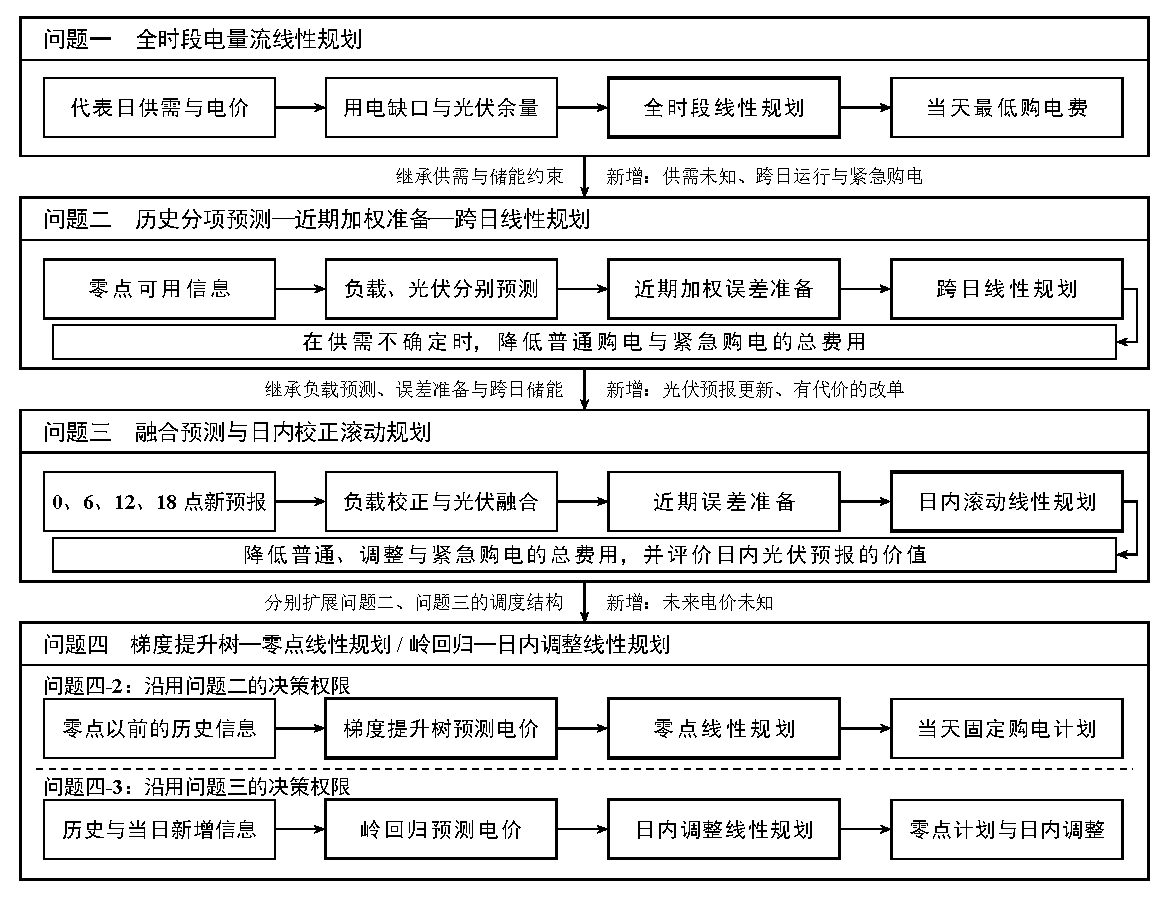
\includegraphics[width=\textwidth]{fig/model.pdf}
\caption{四问整体模型框架}
\label{fig:overall_model_framework}
\end{figure}
